\documentclass[11pt]{article}
\title{%
Skeleton of final report\\\large
\color{white} blank line\\
\color{black}
COMS3\\
Group 9\\
Tracking Interconnected Twitter Links\\
Using Graph Database Neo4j}
\date{2017}
\author{Lindiwe, Clifford, Thomas}

\usepackage[margin=1.5in]{geometry}
\usepackage{hyperref}
\usepackage{graphicx}
\hypersetup{
    colorlinks=true,
    linkcolor=blue,
    filecolor=magenta,      
    urlcolor=blue,
}

\begin{document}
\maketitle
\pagenumbering{gobble}
\newpage
\tableofcontents
\newpage
\pagenumbering{arabic}
\section{Introduction}
\subsection{Overview}
This purpose of this project is to graph Twitter data so that hidden trends and patterns may be revealed.
\subsection{Neo4j}
Neo4j is a relatively new database management system, that distinguishes itself from other systems through its ease of use and its speed. Its was initially launched in 2010, however the stable release was only in June 2017. Its fundamental design is to store data as nodes, edges and attributes. Nodes are connected by edges, both can have any number of attributes.
\subsection{requirements}
To run the code as desired the following programs or packages are required
Neo4j v3.2.4\newline
Python v2.7.13\newline
PyCharm 2017.2.3\newline
TextBlob v0.13.0\newline
Tweepy v3.6.0\newline
py2neo v3.1.2\newline
$\href{https://github.com/TJ721988/SEgroup9/blob/master/Cipher_Queries.txt}{Cipher Queries}(GitHub)\newline 
\href{https://github.com/TJ721988/SEgroup9/blob/master/Twitter_neo.py}{Twitter neo}(GitHub)\newline $
\subsection{Running the code}
The specifics of running the code as desired can be found on $\href{https://github.com/TJ721988/SEgroup9/blob/master/README.md}{\texttt{GitHub in the ReadMe}}$  document
\section{Description}
We import public data from twitter and store it in a Neo4j database. This database is graphically represented through the Neo4j Browser, which shows nodes and connections, in different colours and sizes to highlight and differentiate various things. Filters can be applied to customise or limit what the graph shows. For example only tweets with a certain phrase or hashtag, "\#neo4j", can be shown. This can give an idea about the age, location or gender of people tweeting about Neo4j.

\subsection{Design}

Figure 1 shows a demo of the final look. Big green nodes are people on twitter, labelled by their twitter handle, they share an edge labelled "tweeted" to red nodes, labelled "T" with anything they tweet. Should anyone retweet this tweet, then a "RT" node is created in purple, sharing "retweeted" edges with the original tweet and the retweter. Another edge is created from the retweeter to the original tweeter if they are a follower.
\newline
Figure 2 shows the data process, from Twitter to the final front-end interface. \newline
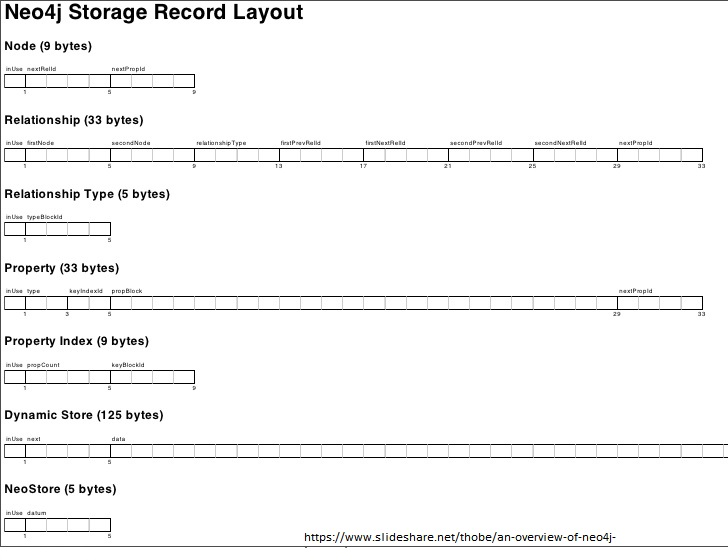
\includegraphics[scale=0.70]{Detail}
Figure 3 shows the basic idea behind the set up of the database.\newline

\includegraphics[scale=0.5]{Graph}\newline
\includegraphics[scale=0.5]{JSON}
We discussed including the location of where the tweet was made, however this is problematic for several reasons
\begin{itemize}
\item Not all users share their location with twitter
\item Different providers share locations differently (3 locations from our testing include, "\#GameofThrones" vs "Basin, WY, United States" vs "Kenya")
\end{itemize}

Discuss sentiment.



\subsection{Back-end}
simple description on what the back-end does and why

\subsection{Front-end}
Front end stuff

\subsection{application}
A tool like this has many applications, certain tweet patters could signal to an account being bot operated, it can be used to find out what a certain age, race, gender, location are tweeting about a certain topic. The first application that pops to mind is targeted advertising, but many more exist.

\subsection{looking forward}
The first improvement we would like to make would be to host the Neo4j database on a server, so that visual designs and templates can be stored for a uniform look. The next would be a script, either through a website or a program to automate the initial set up in Python and pyCharm, so that the user just needs to select his preferences or enter a topic into a search field and the script does the rest and displays the results in the browser.

\section{Members}
who did what




\end{document}